\section{Actividad No 01 – Introduccion a los Sistemas de Control de Versiones} 
¿Que es un Sistema de Control de Versiones?

\begin{itemize}
	\item Un Sistema de Control de Versiones (en adelante SCV), es un software que controla y organiza las distintas revisiones que se realizen sobre uno o varios documentos.
	\\ \\Una  revisión es un cambio realizado sobre un documento,por ejemplo añadir un parrafo, borrar un fragmento o algo similar
	\\EJEMPLO:
	\\Supongamos que cargamos en un SCV el siguiente código fuente:

	\begin{center}
	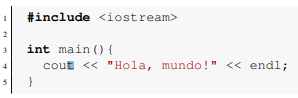
\includegraphics[width=5cm]{./Imagenes/imagen01} 
	\end{center}
	
	\item Se añade al SCV como la revisión 1 del fichero. Una vez añadido, vemos que no compila, ya que nos falta incluir el uso del espacio de nombres, así que lo modificamos:
	
	\begin{center}
	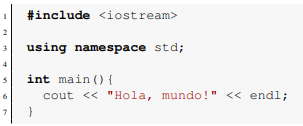
\includegraphics[width=5cm]{./Imagenes/imagen02} 
	\end{center}

	\item Se vuelve a añadir al SCV, ahora como la revisión número 2. De esta forma, se guarda el historial de las distintas modificaciones sobre un fichero, por lo que en cualquier momento podemos restaurar la revisión que queramos de un fichero.
	

\end{itemize}